\section{Grundlagen}

\frame{\frametitle{Agenda}\tableofcontents[currentsection]}
\begin{frame}
	\frametitle{Inductive Logic Programming (ILP)}

	\begin{block}{Was ist Inductive Logic Programming?}
			Die Schnittstelle zwischen Machine Learning und logischer Programmierung
	\end{block}
	\img{process2cut}{Prozessablauf}{}{0.65}
\end{frame}

\begin{frame}
	\frametitle{Logik erster Stufe -- Einführung}

	In \textbf{Logik erster Stufe} besteht die Welt aus
	\begin{itemize}
		\item Objekten  $(Personen, Dingen)$
		\item Prädikaten $(>, <)$
		\item Funktionen $(+, -)$
	\end{itemize}
\end{frame}

\begin{frame}
	\frametitle{Logik erster Stufe -- Einführung}
	\emph{Terme} beschreiben Objekte in der Welt:\\
	\begin{itemize}
		\item Konstanten  ($2$, Chuck Norris)
		\item Variablen   ($x,y, a, \ldots$)
		\item Funktionen von Termen ($add(x,2)$)
	\end{itemize}

	\emph{Grundterme}: Terme ohne Variablen.
	\pause

	\vspace{15pt}
	\emph{Atome} sind kleinstmögliche wahre Ausdrücke
	\begin{itemize}
		\item $predicate(Term_1, \ldots, Term_n)$\\
			Beispiel: is\_human(Pinoccio)
		\item $Term_1 = Term_2$ (Gleicheitsrelation)
	\end{itemize}
	\emph{Literale} sind (negierte) Atome

\end{frame}

\begin{frame}
	\frametitle{Logik erster Stufe -- Syntax}

	\begin{block}{Syntaktische Beschreibung der Welt}
		\begin{align*}
			\text{Konstante} &= \{\text{Zero}\}\\
			\text{Funktionen}  &=\{Succ/1, Plus/2 \}\\
			\text{Prädikate} &=\{even/1, is\_greater/2 \}
		\end{align*}
	\end{block}

\end{frame}

\begin{frame}
	\frametitle{Logik erster Stufe -- Semantik}
	Interpretation $\mathcal{I}$ besitzt eine Grundmenge $\mathcal{M}$
	und bildet Konstanten und Funktionen auf Elemente der Grundmenge ab.

	Prädikate werden auf Wahrheitswerte abgebildet

	\begin{block}{Interpretation}
		\begin{align*}
			\mathcal{M} &= \mathbb{N}_0\\
			\mathcal{I}(Zero) &= 0\\
			\mathcal{I}(Plus(Succ(Zero), Succ(Zero))) = \mathcal{I}(Succ(Succ(Zero)) &=  2\\
			\mathcal{I}(even(Succ(Succ(Zero)))) &= True
		\end{align*}
	\end{block}
\end{frame}

\begin{frame}
	\frametitle{Logik erster Stufe -- Semantik II}
	\begin{block}{Logische Folgerung}
		Man schreibt
		\begin{align*}
			\Gamma \vDash \varphi
		\end{align*}
		Gdw. jede Intepretation $\mathcal{I}$, die alle Formeln
		der Menge $\Gamma$ erfüllt, auch $\varphi$ erfüllt.
	\end{block}
	\begin{bsp}
		\begin{align*}
			\{A \rightarrow B, A\} \vDash B
		\end{align*}
	\end{bsp}
\end{frame}

\begin{frame}
	\frametitle{Horn-Klauseln}
	Horn Clauses: Klausel mit maximal einem positiven Literal.

	\begin{align*}
		\neg C_1 \lor \neg C_2 \lor \ldots \lor \neg C_n  \lor C_{n+1} \Leftrightarrow\\
		C_1 \land C_2 \land \ldots \land C_n  \rightarrow C_{n+1}
	\end{align*}

	ILP verwendet zumeist \textit{definite program clauses } (genau ein positives Literal) vom Typ:

	\begin{align*}
		\underbrace{T}_{\text{head}} \leftarrow \underbrace{L_1, \ldots, L_m}_{\text{body}}
	\end{align*}
	wobei $L_1, \ldots, L_m$ Literale sind und $T$ ein Atom ist.

	Beispiel:
	\begin{align*}
		daughter(X,Y) \Leftarrow female(X), parent(Y, X)
	\end{align*}
\end{frame}

\begin{frame}
	\frametitle{Hypotheseneigenschaften}
	\emph{Gegeben:} Background-Knowledge $(\mathcal{B})$, Menge von positiven $(E^+)$ und negativen
	$(E^-)$ Beispielen.\\
	\emph{Ziel:} Finden einer Hypothese $(\mathcal{H})$, die alle positiven und keine negativen
	Beispiele erfüllt.

	\begin{minipage}{0.5\textwidth}
		\vspace{5pt}
		\underline{Eigenschaften}
		\begin{itemize}
			\item Sufficiency:        $\mathcal{B} \land \mathcal{H} \vDash E^{+}$

				Hypothese $\mathcal{H}$ muss alle positiven Beispiele logisch folgern

			\item Strong consistency: $\mathcal{B} \land \mathcal{H} \land E^{-} \nvDash false$

				$\mathcal{H}$ darf negativen Beispielen nicht widersprechen
		\end{itemize}
	\end{minipage}
	\begin{minipage}{0.45\textwidth}
		\centering
		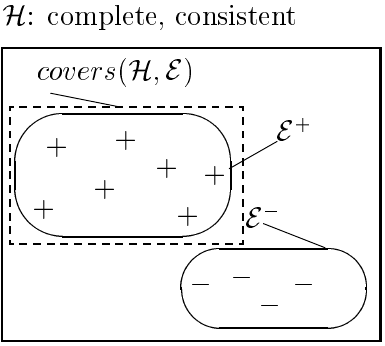
\includegraphics[scale=0.35]{hypothesis_correct}
	\end{minipage}
\end{frame}
%\begin{frame}
%\frametitle{Hypotheseneigenschaften}
%	\emph{Gegeben:} Background-Knowledge $(\mathcal{B})$, Menge von positiven $(E^+)$ und negativen $(E^-)$ Beispielen\\
%	\emph{Ziel:} Finden einer Hypothese $(\mathcal{H})$ die alle positiven und kein negatives Beispiele erfüllt
%\begin{figure}[H]
%	\centering
%	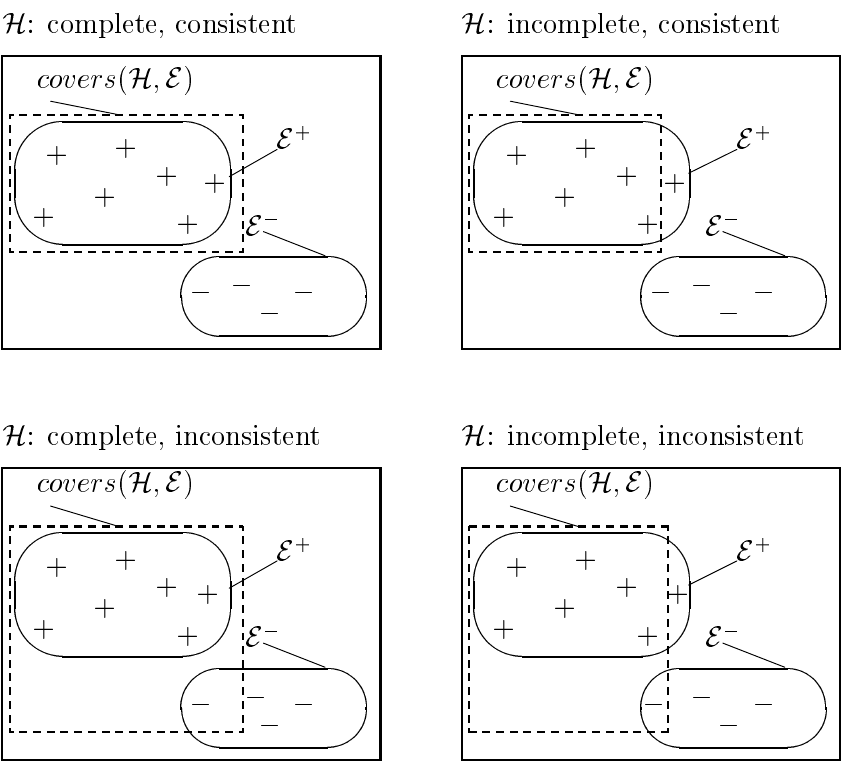
\includegraphics[width=0.5\textwidth]{hypothesis}
%\end{figure}
%\end{frame}
%
%\begin{frame}
%	\frametitle{Gewünschte Hypotheseneigenschaften}
%	\begin{itemize}
%		\item Necessity:          $\mathcal{B} \nvDash E^{+}$
%
%			Beispiele dürfen nicht durch Hintergrundwissen allein schon erklärbar sein
%
%		\item Sufficiency:        $\mathcal{B} \land \mathcal{H} \vDash E^{+}$
%
%			Hypothese $\mathcal{H}$ muss alle positiven Beispiele logisch folgern
%
%		\item Weak consistency:   $\mathcal{B} \land \mathcal{H} \nvDash false$
%
%			$\mathcal{H}$ darf dem Hintergrundwissen nicht widersprechen
%
%		\item Strong consistency: $\mathcal{B} \land \mathcal{H} \land E^{-} \nvDash false$
%
%			$\mathcal{H}$ darf negativen Beispielen nicht widersprechen
%	\end{itemize}
%\end{frame}
